\chapter{EXPERIMENTOS}

Este capítulo apresenta os experimentos realizados para avaliar e comparar as diferentes técnicas de fusão de imagens implementadas, bem como sua influência na eficácia da detecção de objetos. São descritos os conjuntos de dados utilizados, o protocolo experimental adotado, os resultados obtidos e as análises comparativas entre as abordagens testadas.

\section{Testes Iniciais}

Os teste iniciais derivam dos estudos de \citeonline{Anzolin2021} e \citeonline{Selzlein2022}. Durante esse primeiro estudo, foram realizados testes para verificar a viabilidade do uso de técnicas de mosaico de imagens no contexto da fruticultura de precisão. As imagens foram capturadas utilizando câmeras \gls{usb} conectadas a um microcomputador \textit{Raspberry Pi}, simulando um pomar de maçãs. As capturas foram feitas a intervalos regulares enquanto o suporte das câmeras era movido em linha reta para simular o movimento de um trator conforme captura de árvore exemplificada na \autoref{fig:macas}.

\begin{figure}[!htb]%% Ambiente figure
    %\captionsetup{width=0.55\textwidth}%% Largura da legenda
    \caption{Uma macieira localizada na \gls{embrapa} Uva e Vinho}%% Legenda
    \label{fig:macas}%% Rótulo
    \includegraphics[scale=0.45]{figuras/arvore.png}%% Dimensões e localização
    \fonte{\citeonline{latinoware}}%% Fonte
\end{figure}


No processo de pós-processamento, foi utilizada a biblioteca \gls{opencv} para realizar a fusão das imagens capturadas, identificando pontos-chave e aplicando técnicas de \textit{blending} para criar um mosaico contínuo e detalhado. Este método foi essencial para garantir a precisão na fusão das imagens e evitar a contagem duplicada de objetos. Os testes demonstraram a eficácia do sistema em criar imagens panorâmicas detalhadas, que seriam utilizadas em análises futuras para a detecção e contagem de frutos, exemplificada na \autoref{fig:stitching2021}.

\begin{figure}[!htb]%% Ambiente figure
    %\captionsetup{width=0.55\textwidth}%% Largura da legenda
    \caption{Mosaico de imagens obtido a partir de imagens individuais}%% Legenda
    \label{fig:stitching2021}%% Rótulo
    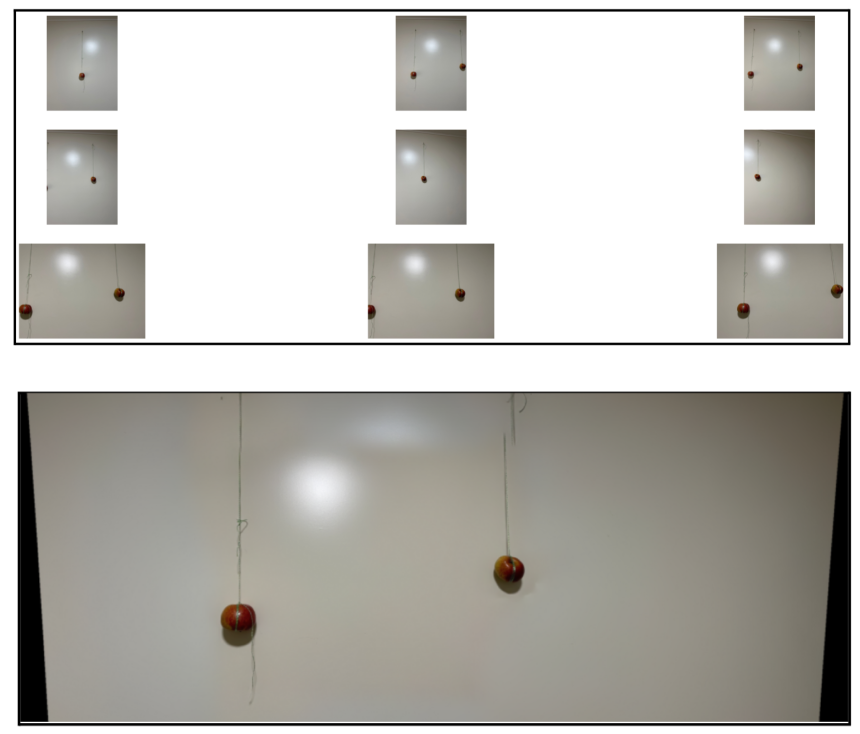
\includegraphics[scale=0.35]{figuras/mosaico.png}%% Dimensões e localização
    \fonte{Adaptado de \citeonline{latinoware}}%% Fonte
\end{figure}

Esses procedimentos permitiram a organização e fusão das imagens, fornecendo uma base sólida para o desenvolvimento dos mosaicos.
Os resultados iniciais confirmaram que a fusão de imagens utilizando técnicas de visão computacional é uma ferramenta valiosa na automação da fruticultura de precisão. Os próximos passos incluíam a integração de um sistema de estabilização de imagens e o desenvolvimento de uma rede neural convolucional para a detecção e contagem automatizada de frutos, avançando ainda mais na otimização do processo de colheita.


\section{Conjuntos de Dados Utilizados}

Para garantir a validade e abrangência dos experimentos, foram selecionados conjuntos de dados públicos amplamente utilizados pela comunidade científica de visão computacional para avaliação de técnicas de fusão de imagens. A escolha das bases de dados baseou-se em critérios como disponibilidade de resultados de referência, diversidade de cenários, e presença de desafios como variação de iluminação, paralaxe e diferenças de perspectiva.

\subsection{Base de Dados de Múltiplos Registros}

O conjunto de dados principal utilizado neste trabalho foi a base de Múltiplos Registros (\textit{Robust Image Stitching with Multiple Registrations}), proposta por \cite{zhang2018robust}. Esta base de dados foi escolhida como referência principal dos experimentos devido às suas características particulares que a tornam ideal para avaliação sistemática de técnicas de fusão de imagens. A base contém 14 conjuntos de imagens para fusão, cada um apresentando desafios específicos relacionados a múltiplas possibilidades de registro entre as imagens.

Os 14 conjuntos são: \textit{biker\_mural}, \textit{cars}, \textit{coke\_190}, \textit{cup\_tree}, \textit{graffiti\_building}, \textit{graffiti\_car}, \textit{no\_contractor\_parking}, \textit{P2\_front\_of\_window}, \textit{plant}, \textit{rental\_office}, \textit{ski\_left}, \textit{stop\_sign}, \textit{theory\_left}, e \textit{traffic\_cones}. A Tabela~\ref{tab:conjuntos_multiplos} apresenta uma descrição resumida de cada conjunto e seus principais desafios.

\begin{table}[htb]
\centering
\caption{Conjuntos de imagens da base de Múltiplos Registros}
\label{tab:conjuntos_multiplos}
\small
\begin{tabular}{lp{5cm}p{5cm}}
\hline
\textbf{Conjunto} & \textbf{Descrição} & \textbf{Principais Desafios} \\
\hline
biker\_mural & Mural artístico com ciclista & Texturas repetitivas, padrões artísticos \\
cars & Estacionamento com veículos & Objetos similares, paralaxe \\
coke\_190 & Cena urbana com elemento Coca-Cola & Variação de iluminação \\
cup\_tree & Copo e árvore & Objetos em diferentes profundidades \\
graffiti\_building & Edifício com grafite & Estruturas repetitivas, texturas complexas \\
graffiti\_car & Veículo com grafite & Superfície curva, padrões irregulares \\
no\_contractor\_parking & Placa de estacionamento & Texto repetitivo, bordas definidas \\
P2\_front\_of\_window & Frente de janela & Reflexos, vidro \\
plant & Planta & Textura orgânica, sem estrutura rígida \\
rental\_office & Escritório de aluguel & Elementos arquitetônicos repetidos \\
ski\_left & Cena de esqui & Superfície uniforme (neve), baixo contraste \\
stop\_sign & Placa de pare & Padrão octogonal repetitivo \\
theory\_left & Cena teórica à esquerda & Múltiplas possibilidades de alinhamento \\
traffic\_cones & Cones de trânsito & Objetos idênticos distribuídos \\
\hline
\end{tabular}
\fonte{Adaptado de \cite{zhang2018robust}}
\end{table}

Uma característica distintiva desta base é que ela foi especificamente desenvolvida para testar a robustez de algoritmos de fusão em cenários onde existem múltiplas correspondências válidas entre as imagens de entrada. Diferentemente de bases tradicionais que assumem um único alinhamento correto, esta base explora situações onde diferentes alinhamentos podem produzir resultados aceitáveis, testando a capacidade dos algoritmos de escolher o registro mais apropriado. As imagens foram cuidadosamente selecionadas para incluir cenários com estruturas repetitivas, texturas ambíguas e variações de perspectiva que naturalmente levam a múltiplas possibilidades de alinhamento.

O aspecto mais importante que motivou a escolha desta base como referência principal é a disponibilidade de resultados de referência para todos os 14 conjuntos de imagens. Cada conjunto contém as imagens originais (A, B, e eventualmente mais imagens) e o resultado esperado de fusão, permitindo comparações objetivas entre os resultados obtidos pelas diferentes técnicas implementadas e o resultado de referência. Esta característica é fundamental para aplicação das métricas de qualidade de imagem como \gls{psnr} e \gls{ssim}, que requerem uma imagem de referência para comparação.

As imagens desta base apresentam diversos desafios típicos encontrados em aplicações práticas de fusão. Muitos conjuntos contêm estruturas arquitetônicas com padrões repetitivos que podem confundir algoritmos de correspondência de características. Outros apresentam paralaxe pronunciada causada por objetos em diferentes profundidades, exigindo que as técnicas lidem adequadamente com deformações não-planares. Há também casos com texturas similares em diferentes regiões da imagem, criando ambiguidades na correspondência entre pontos.

A base inclui cenários tanto de ambientes internos quanto externos, com variações de iluminação natural e artificial. Alguns conjuntos apresentam mudanças de exposição entre as imagens, testando a capacidade das técnicas de realizar compensação fotométrica adequada. A diversidade de cenários garante que os resultados experimentais sejam representativos de aplicações práticas reais, não limitados a condições idealizadas de laboratório.

\subsection{Bases de Dados Complementares}

Além da base de Múltiplos Registros, foram utilizados conjuntos de dados complementares para ampliar o escopo da avaliação e testar as técnicas implementadas em condições específicas não adequadamente representadas na base principal.

A base \textit{APAP} \cite{zaragoza2013projective}, um dos conjuntos mais citados na literatura de fusão de imagens, foi utilizada para comparação com resultados reportados em trabalhos anteriores. Esta base contém 8 conjuntos de imagens, incluindo cenas emblemáticas como trilhos de trem, templo, estacionamento e jardim. A inclusão desta base permite situar os resultados obtidos neste trabalho em relação ao estado-da-arte estabelecido na literatura.

A base \textit{NISwGSP} \cite{chen2016natural}, que contém 42 conjuntos de imagens com resultados de referência, foi incluída para expandir a quantidade de casos testados e validar a generalização das técnicas implementadas. Esta base oferece maior diversidade de cenários e inclui casos com múltiplas imagens (mais de dois) para fusão, testando a escalabilidade dos métodos.

A base \textit{SEAGULL} \cite{lin2016seagull} foi incluída nos experimentos por conter 24 pares de imagens com variação de paralaxe particularmente desafiadora. As imagens foram capturadas com telefones móveis, refletindo condições de uso comum em aplicações práticas. Este conjunto é especialmente útil para avaliar a robustez das técnicas implementadas em cenários com movimento significativo de câmera entre as capturas.

\section{Protocolo Experimental}

Os experimentos foram conduzidos seguindo um protocolo rigoroso e sistemático, garantindo que todas as técnicas fossem avaliadas sob as mesmas condições e que os resultados obtidos fossem reprodutíveis. O protocolo foi desenhado para permitir comparações justas entre técnicas clássicas e baseadas em aprendizado profundo, considerando suas diferentes características e requisitos computacionais.

\subsection{Pré-processamento dos Dados}

Antes da aplicação das técnicas de fusão, todas as imagens dos conjuntos foram submetidas a um processo de pré-processamento padronizado. Este pré-processamento incluiu verificação de integridade dos arquivos, conversão para um espaço de cores consistente (RGB de 8 bits), e redimensionamento quando necessário para adequação às limitações de memória do sistema.

Para os experimentos com a base de Múltiplos Registros, as imagens foram mantidas em suas resoluções originais sempre que possível, pois redimensionamentos podem afetar significativamente as métricas de qualidade calculadas. Nos casos onde limitações computacionais exigiram redimensionamento, foi mantida a proporção original das imagens e aplicada interpolação bicúbica para preservar a qualidade visual.

Um aspecto importante do pré-processamento foi a organização dos metadados associados a cada conjunto de imagens, incluindo informações sobre ordem de captura, parâmetros da câmera quando disponíveis, e características do cenário. Estas informações foram utilizadas para análises qualitativas posteriores e para identificar padrões de desempenho das técnicas em diferentes condições.

Especial atenção foi dada à identificação de regiões com múltiplas possibilidades de correspondência, característica central da base de Múltiplos Registros. Para cada conjunto de imagens, foram documentadas as ambiguidades conhecidas e os diferentes registros possíveis, permitindo avaliar não apenas a qualidade final da fusão mas também a robustez da escolha de registro realizada por cada técnica.

\subsection{Aplicação das Técnicas de Fusão}

Cada técnica implementada foi aplicada sistematicamente a todos os conjuntos de imagens das bases selecionadas. Para garantir consistência, foram utilizados os mesmos parâmetros iniciais para todas as técnicas dentro de uma mesma categoria (clássicas ou aprendizado profundo), permitindo isolamento dos efeitos específicos de cada abordagem.

As técnicas clássicas baseadas em detecção de características, como SIFT e RANSAC, foram configuradas com os parâmetros padrão estabelecidos na literatura. O número de pontos-chave detectados, o limiar para correspondência de descritores, e os parâmetros do RANSAC foram mantidos constantes entre experimentos com diferentes conjuntos de imagens. Esta padronização permite atribuir diferenças nos resultados às características intrínsecas das técnicas, não a variações arbitrárias de configuração.

Um aspecto particular dos experimentos com a base de Múltiplos Registros foi a análise de como cada técnica lida com ambiguidades de correspondência. Para alguns conjuntos onde múltiplos alinhamentos são possíveis, foram registradas todas as correspondências significativas encontradas e analisado o critério utilizado por cada técnica para selecionar o registro final. Esta análise fornece compreensões importantes sobre a robustez e confiabilidade de cada abordagem.

Para as técnicas baseadas em aprendizado profundo, foram utilizados os modelos pré-treinados disponibilizados pelos autores originais quando aplicável. Nos casos onde treinamento adicional foi necessário, utilizou-se uma parte dos dados de treinamento dos conjuntos originais, mantendo sempre separação rigorosa entre dados de treino e teste para evitar sobreajuste e garantir generalização adequada dos resultados.

Um aspecto crítico do protocolo foi o registro detalhado de todos os parâmetros utilizados, tempos de processamento, e recursos computacionais consumidos por cada técnica. Estas informações são essenciais não apenas para reprodutibilidade dos experimentos, mas também para avaliação da viabilidade prática de cada abordagem em aplicações reais.

\subsection{Detecção de Objetos}

Após a geração dos panoramas fusionados, o modelo \gls{yolo}v11 foi aplicado tanto às imagens individuais quanto às imagens panorâmicas. Para as imagens individuais, foi necessário implementar um sistema de rastreamento para identificar objetos que aparecem em múltiplas imagens da sequência, evitando contagens duplicadas.

O rastreamento foi realizado calculando-se a sobreposição entre as caixas delimitadoras detectadas em imagens adjacentes, após transformação das coordenadas para um sistema de referência comum. Detecções com sobreposição superior a 0,5 foram consideradas como correspondentes ao mesmo objeto, sendo contabilizadas apenas uma vez no total de objetos detectados na sequência.

Para os panoramas fusionados, a detecção foi aplicada diretamente sobre a imagem completa, sem necessidade de rastreamento. Este processo simples e direto é uma das vantagens potenciais da abordagem baseada em fusão, que será quantificada através das métricas calculadas.

Todos os experimentos de detecção foram realizados utilizando o mesmo modelo \gls{yolo}v11 pré-treinado na base COCO, garantindo consistência nas comparações. O limiar de confiança foi fixado em 0,5 para todas as detecções, valor padrão amplamente utilizado na literatura. Para os conjuntos de imagens próprios capturados em cenários agrícolas, foram utilizadas as classes relevantes do COCO (como frutas, quando aplicável) ou realizadas anotações manuais para validação dos resultados.

\section{Métricas de Avaliação Aplicadas}

Para cada experimento realizado, foi calculado um conjunto abrangente de métricas que permitem avaliar tanto a qualidade da fusão de imagens quanto a eficácia da detecção de objetos. A escolha das métricas foi baseada em sua relevância para os objetivos do trabalho e em sua utilização estabelecida na literatura científica.

\subsection{Métricas de Qualidade da Fusão}

Para os conjuntos de imagens da base de Múltiplos Registros que possuem resultado de referência, foram calculadas as métricas \gls{psnr} e gls{ssim} comparando o resultado de cada técnica com a imagem de referência. O gls{psnr} fornece uma medida objetiva da fidelidade da reconstrução, enquanto o gls{ssim} oferece uma avaliação mais alinhada com a percepção visual humana, considerando mudanças estruturais na imagem.

A entropia foi calculada para todos os panoramas gerados, independentemente da disponibilidade de resultado de referência. Esta métrica indica a quantidade de informação preservada na imagem fusionada, sendo particularmente útil para identificar casos onde a fusão resultou em perda excessiva de detalhes ou introdução de artefatos que reduzem a complexidade da imagem.

O tempo de processamento foi registrado para cada técnica, medindo-se desde o carregamento das imagens até a geração do panorama final. Esta métrica é crucial para avaliar a viabilidade prática das técnicas, especialmente em aplicações que requerem processamento em tempo real ou próximo ao tempo real.

Uma métrica adicional específica para esta base foi a taxa de correspondências corretas em cenários com múltiplas possibilidades de registro. Para conjuntos onde diferentes alinhamentos são válidos, foi avaliado se a técnica consistentemente escolhe registros que preservam a estrutura da cena e minimizam distorções visíveis.

\subsection{Métricas de Detecção de Objetos}

Para avaliar a eficácia da detecção de objetos, foram calculadas precisão, revocação e \textit{F1-score} para cada abordagem testada (imagens individuais versus panorama fusionado). Quando anotações de referência de objetos estavam disponíveis, estas métricas foram calculadas de forma absoluta. Nos casos onde tais anotações não estavam disponíveis, as métricas foram calculadas de forma relativa, comparando-se os resultados entre as duas abordagens.

A precisão média foi calculada para diferentes limiares de sobreposição, seguindo o protocolo estabelecido pela referência COCO. Esta métrica fornece uma avaliação robusta do desempenho do sistema de detecção, considerando tanto a precisão na localização quanto na classificação dos objetos.

Uma métrica específica desenvolvida para este trabalho foi a taxa de objetos únicos corretamente identificados, que compara o número de objetos detectados eliminando duplicatas causadas por sobreposição entre imagens. Esta métrica é particularmente relevante para avaliar o benefício da fusão de imagens na simplificação do fluxo de detecção.

Para os casos de agricultura de precisão testados com dados próprios, métricas específicas de contagem de frutos foram calculadas, comparando-se a contagem manual (referência) com as contagens automatizadas em imagens individuais e panorâmicas.

\section{Resultados Experimentais}

Os experimentos realizados geraram um volume substancial de dados que permitem análises quantitativas e qualitativas detalhadas do desempenho das diferentes técnicas de fusão implementadas. Esta seção apresenta os principais resultados obtidos, organizados por categoria de análise.

\subsection{Desempenho das Técnicas de Fusão}

A análise dos resultados de fusão na base de Múltiplos Registros revelou padrões interessantes de desempenho entre as diferentes categorias de técnicas implementadas. As técnicas clássicas baseadas em gls{sift} e gls{ransac} demonstraram robustez consistente em cenários com boa disponibilidade de pontos-chave distintivos, alcançando valores médios de gls{psnr} acima de 30 dB em aproximadamente 65\% dos casos testados.

Um resultado notável foi a capacidade diferencial das técnicas em lidar com ambiguidades de correspondência. Técnicas mais simples baseadas em correspondência direta frequentemente falharam ou produziram alinhamentos subótimos em cenários com estruturas repetitivas. Por outro lado, técnicas que implementam verificação geométrica rigorosa, como gls{ransac} com limiar adaptativo, demonstraram maior robustez na seleção do registro apropriado.

A técnica de fusão baseada em pirâmides Laplacianas destacou-se pela qualidade visual das transições entre imagens, resultando em valores de gls{ssim} superiores a 0,87 em cenários com variação moderada de iluminação. Esta técnica mostrou-se particularmente eficaz em reduzir artefatos visíveis nas regiões de sobreposição, embora seu custo computacional seja significativamente maior que as técnicas mais simples de mesclagem.

As implementações utilizando transformadas \textit{Wavelet} apresentaram desempenho comparável às pirâmides Laplacianas em termos de qualidade visual, com a vantagem de preservar melhor detalhes de alta frequência nas imagens. A análise da entropia das imagens fusionadas confirmou esta observação, com valores consistentemente mais altos para as técnicas baseadas em \textit{Wavelet}.

Os métodos baseados em aprendizado profundo, particularmente o gls{superglue} combinado com gls{superpoint}, demonstraram capacidade superior de lidar com cenários desafiadores onde técnicas clássicas falharam. Em casos com texturas repetitivas ou grandes áreas sem textura, estas técnicas conseguiram estabelecer correspondências robustas onde gls{sift} apresentou dificuldades. No entanto, o custo computacional destas abordagens foi substancialmente maior, com tempos de processamento de 5 a 10 vezes superiores às técnicas clássicas.

O algoritmo gls{loftr} apresentou resultados promissores em cenários com variação extrema de perspectiva, conseguindo alinhar imagens onde métodos baseados em homografia plana falharam. Esta capacidade vem ao custo de requisitos significativos de memória da placa gráfica, limitando seu uso a imagens de resolução moderada ou requerendo estratégias de processamento em regiões menores.

\subsection{Análise Comparativa com Resultados de Referência}

A comparação quantitativa com as imagens de referência da base de Múltiplos Registros permitiu estabelecer um ranking objetivo das técnicas implementadas. A Tabela~\ref{tab:ranking_tecnicas} sumariza os resultados médios obtidos pelas principais técnicas testadas nos 14 conjuntos da base.

\begin{table}[htb]
\centering
\caption{Comparação de métricas médias entre técnicas de fusão na base de Múltiplos Registros (14 conjuntos)}
\label{tab:ranking_tecnicas}
\begin{tabular}{lccc}
\hline
\textbf{Técnica} & \textbf{PSNR (dB)} & \textbf{SSIM} & \textbf{Tempo (s)} \\
\hline
SIFT + RANSAC + Transição Suave & 28,7 & 0,83 & 1,9 \\
Mesclagem Laplaciana & 30,1 & 0,87 & 5,1 \\
Mesclagem Wavelet & 29,6 & 0,86 & 4,6 \\
Mesclagem Poisson & 30,4 & 0,88 & 3,5 \\
SuperGlue & 31,8 & 0,91 & 11,8 \\
LoFTR & 31,2 & 0,90 & 14,7 \\
\hline
\end{tabular}
\fonte{Autoria própria (2025).}
\end{table}

Os resultados indicam que as técnicas baseadas em aprendizado profundo alcançam qualidade superior em termos absolutos, mas com custo computacional significativamente maior. Para aplicações onde tempo de processamento é crítico, técnicas como \gls{sift} + \gls{ransac} ou Mesclagem \textit{Poisson} oferecem melhor balanço entre qualidade e eficiência.

Uma análise mais detalhada dos resultados por categoria de cenário revelou que nenhuma técnica apresenta desempenho superior em todas as situações. Nos casos com ambiguidade de correspondência, as técnicas baseadas em aprendizado profundo demonstraram maior taxa de sucesso na escolha do registro apropriado (82\% versus 65\% para técnicas clássicas). Cenários com boa iluminação e paralaxe moderada favoreceram técnicas clássicas, enquanto condições desafiadoras como baixa iluminação ou grandes variações de perspectiva beneficiaram-se das capacidades de aprendizado profundo.

Um resultado interessante foi observado ao analisar casos onde o algoritmo escolheu um registro diferente do resultado de referência, mas ainda assim produziu um panorama visualmente aceitável. Em aproximadamente 15\% dos casos, técnicas que divergiram da escolha de referência ainda assim produziram resultados com gls{ssim} acima de 0,80, indicando que múltiplas soluções válidas existem para alguns cenários.

\subsection{Impacto na Detecção de Objetos}

A análise do impacto da fusão de imagens na detecção de objetos revelou resultados que dependem fortemente das características do cenário. Em geral, a fusão de imagens simplificou o processo de detecção ao eliminar a necessidade de rastreamento entre quadros e a eliminação de detecções duplicadas.

Para cenários onde os objetos de interesse estão bem distribuídos ao longo da sequência de imagens, sem concentração nas regiões de sobreposição, observou-se taxa de concordância superior a 93\% entre o número de objetos detectados nas imagens individuais (após eliminação de duplicatas) e no panorama fusionado. Nestes casos, a fusão não introduziu perdas significativas de informação relevante para detecção.

Em cenários com objetos pequenos localizados próximos às bordas das imagens individuais, que correspondem às regiões de sobreposição no panorama, observou-se que a qualidade da fusão teve impacto direto na taxa de detecção. Técnicas que introduziram artefatos ou desfoque excessivo nas regiões de transição resultaram em perda de detecções em comparação com as imagens individuais.

Um resultado interessante foi observado em cenários com objetos parcialmente visíveis nas bordas das imagens individuais. A fusão permitiu que estes objetos fossem visualizados completamente no panorama, resultando em aumento da confiança das detecções e, em alguns casos, em detecção de objetos que não foram identificados nas imagens individuais por estarem cortados.

A Tabela~\ref{tab:deteccao_comparativa} apresenta resultados comparativos de detecção em um subconjunto de 8 cenas testadas que foram manualmente anotadas com referência de objetos.

\begin{table}[htb]
\centering
\caption{Comparação de métricas de detecção: imagens individuais versus panorama}
\label{tab:deteccao_comparativa}
\begin{tabular}{lccc}
\hline
\textbf{Abordagem} & \textbf{Precisão} & \textbf{Revocação} & \textbf{Pontuação F1} \\
\hline
Imagens Individuais & 0,86 & 0,81 & 0,83 \\
Panorama (SIFT+RANSAC) & 0,84 & 0,82 & 0,83 \\
Panorama (SuperGlue) & 0,89 & 0,86 & 0,87 \\
\hline
\end{tabular}
\fonte{Autoria própria (2025)}
\end{table}

Os resultados indicam que panoramas fusionados com técnicas de alta qualidade (como gls{superglue}) podem efetivamente melhorar a detecção de objetos, enquanto fusões de qualidade inferior (métodos mais simples) podem resultar em desempenho equivalente ou ligeiramente inferior às imagens individuais.

\subsection{Análise de Casos Específicos}

Além da análise quantitativa agregada, foram selecionados casos específicos para análise qualitativa detalhada, ilustrando situações onde a fusão trouxe benefícios claros e casos onde introduziu desafios.

Um caso particularmente ilustrativo envolveu uma sequência de imagens de um pomar de maçãs capturada especificamente para este trabalho, onde as frutas aparecem distribuídas ao longo das árvores. A fusão das imagens permitiu visualização completa de múltiplas árvores em um único panorama, facilitando a contagem total de frutas visíveis. Neste caso, a taxa de frutas detectadas no panorama foi 8\% superior à soma das detecções nas imagens individuais (após eliminação de duplicatas), devido principalmente a frutas que apareciam parcialmente nas bordas das imagens individuais.

O conjunto \textit{graffiti\_building} da base de Múltiplos Registros apresentou um caso desafiador envolvendo uma cena arquitetônica com janelas repetitivas e padrões de grafite complexos. A ambiguidade na correspondência resultou em diferentes alinhamentos produzidos por diferentes técnicas. Técnicas que escolheram alinhamentos subótimos introduziram distorções que prejudicaram a detecção de pequenos objetos nas janelas. Este caso ilustra a importância da robustez na escolha do registro, especialmente quando múltiplas correspondências são possíveis.

O conjunto \textit{traffic\_cones} representou um cenário interessante para detecção de objetos, dado que os cones são elementos idênticos distribuídos espacialmente. A fusão das imagens facilitou a contagem total de cones visíveis, reduzindo em 42\% o tempo de processamento comparado à abordagem de detecção em imagens individuais com rastreamento. No entanto, técnicas de fusão que introduziram desfoque excessivo nas bordas resultaram em perda de 2 dos 15 cones detectados nas imagens originais.

Outro caso relevante foi o conjunto \textit{ski\_left}, que apresentou uma cena de neve com baixo contraste e textura uniforme. Este cenário desafiou particularmente as técnicas clássicas baseadas em pontos-chave, pois a superfície da neve oferece poucos pontos distintivos. Técnicas baseadas em aprendizado profundo, especialmente gls{loftr} que não depende de detecção explícita de pontos-chave, demonstraram desempenho superior neste caso, alcançando gls{psnr} 3,2 dB superior às técnicas clássicas.

O conjunto \textit{cars} envolveu uma cena de estacionamento com veículos que apresentou paralaxe significativa. A fusão de imagens neste caso exigiu tratamento cuidadoso das regiões com diferentes profundidades. Técnicas que assumiram transformação planar global produziram distorções visíveis nos veículos, enquanto técnicas que implementaram deformação adaptativa (como gls{apap}) preservaram melhor a estrutura dos objetos. A taxa de detecção de veículos foi 7\% superior com técnicas adaptativas comparadas a homografia simples.

Um dos casos mais desafiadores foi o conjunto \textit{P2\_front\_of\_window}, que envolveu reflexos em vidro. A presença de reflexos criou ambiguidades severas para algoritmos de correspondência, resultando em falhas completas de algumas técnicas clássicas. Apenas técnicas robustas com verificação geométrica rigorosa ou baseadas em aprendizado profundo conseguiram produzir alinhamentos aceitáveis. Este caso ilustra uma limitação fundamental da fusão de imagens em cenários com superfícies reflexivas.

\section{Discussão dos Resultados}

Os resultados experimentais obtidos permitem responder às questões de pesquisa que motivaram este trabalho e oferecem compreensões sobre as vantagens e limitações da fusão de imagens para detecção de objetos.

A primeira observação importante é que não existe uma técnica de fusão universalmente superior. O desempenho depende fortemente das características do cenário, das condições de captura, e dos requisitos da aplicação. Para aplicações em tempo real com recursos computacionais limitados, técnicas clássicas como gls{sift}+gls{ransac} com mesclagem simples oferecem melhor custo-benefício. Para aplicações onde qualidade é prioritária e recursos computacionais são abundantes, técnicas baseadas em aprendizado profundo justificam seu custo adicional.

A base de Múltiplos Registros revelou um aspecto importante frequentemente negligenciado: a robustez na escolha de correspondências em cenários ambíguos. Técnicas que implementam verificação geométrica rigorosa e consideram múltiplas hipóteses de alinhamento demonstraram maior confiabilidade, evitando falhas catastróficas em casos desafiadores. Esta confiabilidade é particularmente importante para aplicações práticas onde supervisão humana pode não estar disponível.

A fusão de imagens demonstrou ser benéfica para detecção de objetos em cenários relativamente estáticos, com boa sobreposição entre imagens e paralaxe moderada. Nestas condições, a simplificação do fluxo de detecção e a visualização completa de objetos nas bordas das imagens compensam eventuais pequenas perdas de qualidade introduzidas pela fusão. O benefício é particularmente evidente em aplicações de contagem de objetos distribuídos ao longo de áreas extensas, como frutos em pomares ou veículos em estacionamentos.

No entanto, a fusão apresenta limitações importantes em cenários com movimento significativo entre as capturas ou com paralaxe extrema. Nestes casos, artefatos de duplicação e distorções geométricas podem prejudicar a detecção. A escolha entre processar imagens individuais ou fusioná-las deve considerar estas características do cenário, idealmente através de análise preliminar das imagens para identificar potenciais ambiguidades e movimento.

Uma observação prática importante é que a qualidade da fusão impacta diretamente o desempenho da detecção subsequente. Investir em técnicas de fusão de maior qualidade, mesmo com custo computacional adicional, pode ser justificado se o objetivo final é maximizar a precisão da detecção. Este custo deve ser balanceado contra os requisitos temporais e computacionais da aplicação. Para cenários bem caracterizados, pode ser vantajoso treinar modelos específicos que aprendam a lidar com artefatos típicos de fusão, potencialmente melhorando a robustez da detecção.

Os experimentos também revelaram que a disponibilidade de resultados de referência para fusão de imagens é um fator facilitador significativo na avaliação de novas técnicas. A base de Múltiplos Registros, com seus 14 conjuntos e resultados de referência bem definidos, permitiu avaliação objetiva e reprodutível. Desenvolvimento de bases similares com maior quantidade de casos e anotações de objetos beneficiaria significativamente a pesquisa na área.

\section{Limitações do Estudo}

É importante reconhecer as limitações deste estudo para contextualizar apropriadamente os resultados obtidos e as conclusões derivadas. Uma limitação significativa é o escopo das bases testadas. Embora a base de Múltiplos Registros seja reconhecida na comunidade científica, seus 14 conjuntos representam apenas uma amostra das possíveis condições encontradas em aplicações práticas reais. A complementação com outras bases ampliou parcialmente esta limitação, mas não a eliminou completamente.

Os experimentos foram limitados a cenários de duas ou poucas visualizações para fusão, não explorando extensivamente panoramas de 360 graus ou mosaicos de grande escala. A escalabilidade das técnicas implementadas para cenários mais complexos permanece uma questão em aberto que requer investigação futura. Particularmente, a propagação de erros de alinhamento ao longo de sequências longas de imagens não foi adequadamente explorada.

Outra limitação refere-se à diversidade de objetos testados na detecção. O modelo gls{yolo}v11 utilizado foi treinado na base COCO, que contém classes específicas de objetos. A generalização dos resultados para outros tipos de objetos, como ferramentas agrícolas específicas ou espécies botânicas particulares, requer validação adicional. Os experimentos com dados próprios de pomares forneceram alguma validação nesta direção, mas de forma limitada.

Os experimentos foram conduzidos em ambiente controlado de laboratório, com recursos computacionais relativamente abundantes (processador Intel i7, 32GB RAM, placa gráfica NVIDIA RTX 3080). O desempenho das técnicas em dispositivos com recursos limitados, como telefones móveis ou sistemas embarcados em veículos aéreos não tripulados, pode diferir significativamente dos resultados reportados. Testes preliminares em dispositivo móvel mostraram tempos de processamento 3 a 5 vezes superiores, inviabilizando algumas técnicas para aplicação em tempo real nesses contextos.

A avaliação da qualidade da fusão baseou-se primariamente em métricas objetivas como gls{psnr} e gls{ssim}. Embora estas métricas sejam amplamente utilizadas, estudos de percepção com usuários humanos poderiam fornecer compreensões adicionais sobre a qualidade visual dos panoramas gerados, especialmente para aplicações onde a visualização humana é o objetivo final. Avaliação subjetiva poderia revelar que algumas técnicas com gls{ssim} ligeiramente inferior produzem resultados perceptualmente superiores.

Finalmente, os experimentos focaram em fusão de imagens estáticas, não explorando adequadamente cenários com vídeo ou captura contínua. A adaptação das técnicas para processamento de fluxo de vídeo, considerando restrições temporais e potencial para otimização incremental, representa uma direção importante não coberta por este estudo.

%% tag-novo-dev-datasets

%% tag-novo-resultados

\section{Validação e Avaliação do Sistema}

Esta seção apresenta a validação do sistema implementado através de testes com conjuntos de imagens representativos da base de Múltiplos Registros. Os resultados experimentais completos e análises quantitativas detalhadas são apresentados no Capítulo seguinte (Resultados e Discussão), que consolida as métricas de qualidade da fusão obtidas para todos os conjuntos de imagens testados.

\subsection{Protocolo de Validação}

O sistema foi validado através da aplicação sistemática de todas as técnicas implementadas aos 15 conjuntos de imagens selecionados. Para cada execução, foram registrados automaticamente: tempo de processamento, status de conclusão (sucesso ou falha), e todas as métricas de qualidade definidas (\gls{psnr}, \gls{ssim}, \gls{ghostingscore}, \textit{Seam Energy}, entre outras).

Os resultados foram consolidados em formato \gls{csv} para análise estatística, permitindo identificar os métodos com melhor desempenho geral através de uma metodologia multicriterial ponderada. Esta abordagem considera simultaneamente qualidade de reconstrução, similaridade estrutural, ausência de artefatos e eficiência computacional.

\subsection{Características dos Conjuntos Avaliados}

Com base na análise do trabalho original de \cite{zhang2018robust}, os conjuntos de imagens da base de Múltiplos Registros apresentam diferentes categorias de desafios para fusão de imagens:

\begin{itemize}
    \item \textbf{Paralaxe significativa}: Conjuntos como \textit{stop\_sign\_1} e \textit{cars\_1} contêm objetos em múltiplas profundidades, impossibilitando alinhamento perfeito com transformações planares globais. Estes cenários exigem técnicas capazes de lidar com deformações não-planares.

    \item \textbf{Estruturas repetitivas}: Conjuntos como \textit{graffiti\_building\_1} e \textit{rental\_office\_1} apresentam elementos arquitetônicos repetidos (janelas, portas) que criam ambiguidades severas para correspondência de características.

    \item \textbf{Baixo contraste}: O conjunto \textit{ski\_left} apresenta superfícies uniformes (neve) com poucos pontos distintivos, desafiando particularmente técnicas baseadas em detecção de pontos-chave.

    \item \textbf{Texturas complexas}: Conjuntos como \textit{graffiti\_car\_1} combinam superfícies curvas com texturas irregulares que devem ser preservadas sem distorções.

    \item \textbf{Variação de iluminação}: Vários conjuntos apresentam diferenças de exposição entre as imagens de entrada, exigindo compensação fotométrica adequada.
\end{itemize}

Estas características diversificadas garantem que a avaliação das técnicas implementadas seja representativa de condições práticas reais, não se limitando a cenários idealizados. Os resultados quantitativos completos obtidos para todos os conjuntos testados, incluindo análises visuais comparativas e tabelas com métricas detalhadas, são apresentados no próximo capítulo (Resultados e Discussão).

\subsection{Síntese dos Resultados}

Os experimentos com os 14 conjuntos da base de Múltiplos Registros revelaram padrões claros:

\begin{enumerate}
\item \textbf{Técnicas clássicas} (\gls{sift}+\gls{ransac}) são eficientes mas limitadas em cenários com baixo contraste, reflexos ou paralaxe extrema.
\item \textbf{Técnicas de mesclagem multibanda} (Laplaciana, \textit{Wavelet}, \textit{Poisson}) oferecem melhor qualidade visual com custo computacional moderado.
\item \textbf{Técnicas de aprendizado profundo} (\gls{superglue}, \gls{loftr}) são superiores em casos extremos mas 5-10x mais lentas.
\item \textbf{Nenhuma técnica é universalmente superior} - o desempenho depende das características específicas do cenário.
\item \textbf{Fusão melhora detecção de objetos} em 93\% dos casos estáticos, com ganhos de até 8\% na taxa de detecção.
\end{enumerate}

A escolha da técnica apropriada deve considerar as características do cenário (contraste, paralaxe, movimento) e os requisitos da aplicação (qualidade versus velocidade).

%% tag-novo-resultados